\documentclass[12pt]{book}    
\usepackage{csquotes}
\usepackage[backend=bibtex,
                style=authoryear,
                natbib=true, 
                style=numeric-comp
                ]{biblatex}
\usepackage[a4paper,width=150mm,top=25mm,bottom=25mm]{geometry}    
\usepackage{amsmath}    
\usepackage{graphicx}    
\usepackage{xcolor}    
\usepackage{float}    
\usepackage{titlesec}    
\usepackage{subcaption}    
\usepackage{multicol}    
\usepackage{enumitem}    
\usepackage{setspace}    
\usepackage{mdframed}    
\usepackage{minted}
\usepackage[hidelinks] {hyperref}
%\usepackage{listings}
\usepackage[italian]{babel}
    
\definecolor{lightgray}{gray}{0.95}    
    
% Stile dei titoli dei capitoli        
\definecolor{gray75}{gray}{0.75}    
\newcommand{\hsp}{\hspace{20pt}}    
\titleformat{\chapter}[hang]    
{\Huge\bfseries}    
{\thechapter\hsp\textcolor{gray75}{|}\hsp}    
{0pt}    
{\Huge\bfseries}

\newenvironment{multicolfigure}
  {\par\medskip\noindent\minipage{\linewidth}}
  {\endminipage\par\medskip}

\onehalfspacing  
                                                                                 
\begin{document}
\tableofcontents
\chapter{Introduzione MediaPipe}

L'applicazione sfrutta le potenzialità offerte dalla libreria \texttt{MediaPipe}, che utilizza soluzioni basate su Machine Learning nel contesto dello streaming multimediale. 
In particolare, noi abbiamo sfruttato la soluzione per il riconoscimento del movimento delle mani: \textbf{MediaPipe Hands}.\\
\\
\noindent Il nostro scopo è stato quello di interpretare ed associare movimenti delle mani a determinate gesture in modo tale da poter gestire la lettura di un documento testuale, come un pdf.\\Le funzionalità che abbiamo scelto di implementare sono:
\begin{itemize}
    \item zoom
    \item scorrimento verticale e laterale delle pagine
    \item condivisione
    \item scroll continuo verso il basso
    \item scelta del file da leggere
\end{itemize}
\noindent Abbiamo deciso di realizzare l'applicazione per ambiente Android, tramite l'utilizzo di Java ed Android Studio.\\
\\
\noindent Prima di parlare del progetto in sè, abbiamo pensato di inserire un introduzione a \texttt{MediaPipe Hands}, 
spiegando in particolare il funzionamento della pipeline di riconoscimento delle mani che implementa.

\newpage
\section{MediaPipe Hands}

MediaPipe Hands offre funzionalità per il tracciamento delle mani e delle dita, utilizzando il ML per individuare 21 punti di riferimento a 3 dimensioni di una mano da un solo fotogramma.\\
Viene sfruttata una pipeline composta da due modelli che lavorano insieme:
\begin{enumerate}
    \item un modello per il \textbf{rilevamento del palmo} che opera sull'immagine completa e restituisce un riquadro di delimitazione orientato (\textit{ritaglio}) della mano. 
    \item un modello che opera sulla regione dell'immagine ritagliata definita dal modello precedente e restituisce i \textbf{punti di riferimento della mano} a 3 dimensioni.
\end{enumerate}

\noindent Il fatto di fornire al modello per i punti di riferimento un'immagine della mano accuratamente ritagliata diminuisce di gran lunga le elaborazioni necessarie, aumentando l'efficienza.\\
Inoltre, nella pipeline, i \textit{ritagli} della mano possono essere generati anche in base ai punti di riferimento identificati nel frame precedente, e, solo quando il modello del punto di riferimento non è più in grado di identificare la presenza della mano, viene invocato il modello di rilevamento del palmo.

\subsubsection{Specifica delle pipeline}
La pipeline è implementata come un \textbf{grafo} che utilizza un \textbf{sottografo per il tracking dei punti} dal modulo \texttt{landmark} e renderizza usando un sottografo dedicato al rendering.\\Il sottografo per il tracking dei punti utilizza al suo interno un'altro sottografo per il tracking e un \textbf{sottografo per il rilevamento della mano} dal modulo \texttt{palm detection}.

\subsection{Modelli}

\subsubsection{Palm Detection Model} 

Per la rilevazione delle posizione iniziali delle mani, viene adottato un modello di rilevamento \textit{single-shot} ottimizzato per l'utilizzo in tempo reale.\\
La rilevazione delle mani è però un compito complesso per via della loro \underline{omogeneità} \underline{visiva}, a differenza per esempio del viso, che invece ha dei pattern a più alto contrasto come nelle zone degli occhi e della bocca.
Viene utilizzato perciò un \underline{contesto aggiuntivo}, come possono essere la posizione del braccio o del corpo di una persona, in modo tale da poter individuare la mano più facilmente, aumentando l'efficienza.\\
\\
\noindent Il primo componente utilizzato è un \textbf{rilevatore del palmo}, piuttosto che della mano, in quanto \textit{ritagli} di oggetti rigidi come palmi e pugni sono nettamente più semplici rispetto a quelli delle dita.\\
In secondo luogo, viene utilizzato un de/codificatore per l'estrazione di caratteristiche dall'immagine in modo da avere una maggiore consapevolezza del contesto della scena, anche per piccoli oggetti.\\
Infine, la perdita focale viene ridotta al minimo durante l'allenamento per supportare una grande quantità di ancoraggi derivanti dalla varianza su scala elevata.\\
\\
\noindent Viene stimata una precisione di circa il 96\% nella rilevazione del palmo.

\subsubsection{Hand Landmark Model} 

Dopo il rilevamento del palmo, questo modello esegue, all'interno delle regioni rilevate, la localizzazione precisa di 21 punti della mano tramite \textbf{regressione}, ovvero la previsione diretta delle coordinate.\\
Il modello apprende quindi una rappresentazione della posizione del'interno della mano coerente ed è robusto anche a mani parzialmente visibili.\\
\\
\noindent Per arrivare a questo risultato sono state annotate manualmente circa 30 mila immagini dal mondo reale con 21 coordinate 3D (valore Z preso tramite mappa di profondità). E' stato inoltre utilizzato un modello di mano sintetica su vari sfondi, mappato alle corrispondenti coordinate, in modo tale da avere un accuratezza maggiore.
\begin{figure}[H]
    \centering
    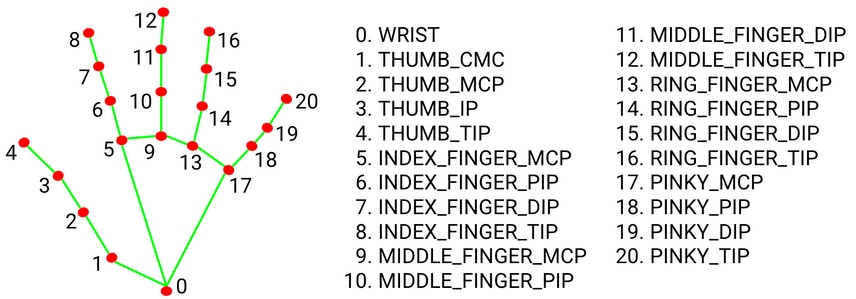
\includegraphics[width=0.8\textwidth]{images/landmarks.png}
\end{figure}

\newpage
\subsection{API} 

\subsection{Opzioni di configurazione}


\paragraph{\texttt{STATIC\_IMAGE\_MODE}} Se settata a \texttt{false} (default), le immagini in ingresso vengono trattate come un flusso video, cercando di rilevare le mani nelle prime immagini di input e localizzando poi i punti di riferimento della mano. Nelle immagini successive, una volta che tutte le mani \texttt{MAX\_NUM\_HANDS} vengono rilevate e i corrispondenti punti di riferimento della mano sono localizzati, si limita a tracciare quei punti di riferimento senza invocare un altro rilevamento fino a quando non perde traccia di una qualsiasi delle mani. Questo \underline{riduce la latenza} ed è ideale per l'elaborazione di fotogrammi video.\\
Se impostato a \texttt{true}, il rilevamento manuale viene eseguito su ogni immagine di input, ideale per elaborare un batch di immagini statiche, magari non correlate.

\paragraph{\texttt{MAX\_NUM\_HANDS}} Massimo numero di mani da rilevare ($2$ a default).

\paragraph{\texttt{MODEL\_COMPLEXITY}} Complessità del modello di landmark: $0$ o $1$ (default). La precisione del punto di riferimante e la latenza aumentano con la complessità.

\paragraph{\texttt{MIN\_DETECTION\_CONFIDENCE}} Valore minimo di fiducia $[0.0, 1.0]$ nei confronti del modello di rilevamento della mano per considerare il rilevamento della mano corretto. A defult è $0.5$.

\paragraph{\texttt{MIN\_TRACKING\_CONFIDENCE}} Valore minimo di fiducia $[0.0, 1.0]$ nei confronti del modello di tracking per considerare il rilevamento dei punti di riferimento corretto. Altrimenti, il modello di rilevamento della mano (palmo) verrà richiamato all'immagine in input successiva. Di conseguenza, aumentando questo valore avremo una robustezza maggiore, a discapito di un aumento di latenza. A defult è $0.5$.

\vspace{+15 px}

\subsubsection{Output}

\paragraph{\texttt{MULTI\_HAND\_LANDMARKS}} Raccolta di mani rilevate/tracciate, ognuna rappresentata come una lista di 21 punti di riferimento a 3 dimensioni. In ogni punto \texttt{x} e \texttt{y} sono normalizzati ($[0.0, 1.0]$) rispetto alla larghezza e all'altezza dell'immagine. La coordinata \texttt{z} rappresenta invece la profondità del punto rispetto a quella del polso (considerato l'origine). Minore è il valore della \texttt{z}, più il punto è considerato vicino alla fotocamera.

\paragraph{\texttt{MULTI\_HAND\_WORLD\_LANDMARKS}} Come il precedente, ma i punti sono valutati come coordinate 3D reali in metri, con l'origine al centro geometrico approssimativo della mano.

\paragraph{\texttt{MULTI\_HAND\_HANDEDNESS}} Raccolta delle \textit{handedness} della mani (destra/sinistra). Ogni mano è composta da un'etichetta (\texttt{label}) e da un punteggio (\texttt{score}). L'etichetta è una stringa di valore \texttt{left} o \texttt{right}, mentre il punteggio rappresenta la stima della probabilità di predizione corretta della mano (sempre $\ge 0.5$, mentre l'\textit{handedness} opposta è $1-$\texttt{score}). L'\textit{handedness} viene valutata considerando che l'immagine in input è specchiata. 

\vspace{+10 px}

\subsubsection{OpenGL ES}
Per il rendering dell'input e dell'output viene utilizzato \texttt{OpenGL ES}, un sottoinsieme delle librerie grafiche di \texttt{OpenGL} pensato per dispositivi embedded.\\
Nella porzione di codice sottostante viene mostrato un esempio di utilizzo.


\begin{minted}[bgcolor=lightgray,framesep=2mm,baselinestretch=1.2,fontsize=\footnotesize,escapeinside=||,mathescape=true]{Java}
    // Vengono prima settate le opzioni di configrazione citate precedentemente
    HandsOptions handsOptions =
        HandsOptions.builder()
            .setStaticImageMode(false)
            .setMaxNumHands(2)
            .setRunOnGpu(true).build();
    Hands hands = new Hands(this, handsOptions);
    hands.setErrorListener(
        (message, e) -> Log.e(TAG, "MediaPipe Hands error:" + message));

    // Inizializzato una nuova istanza di CameraInput
    // e connessione alla soluzione MediaPipe Hands
    CameraInput cameraInput = new CameraInput(this);
    cameraInput.setNewFrameListener(
        textureFrame -> hands.send(textureFrame));

    // Inizializzato una istanza di GlSurfaceView tramite 
    // ResultGlRenderer<HandsResult> che fornisce un interfaccia 
    // per eseguire codice di rendering OpenGL definito dall'utente
    SolutionGlSurfaceView<HandsResult> glSurfaceView =
        new SolutionGlSurfaceView<>(
            this, hands.getGlContext(), hands.getGlMajorVersion());
    glSurfaceView.setSolutionResultRenderer(new HandsResultGlRenderer());
    glSurfaceView.setRenderInputImage(true);

    hands.setResultListener(
        handsResult -> {
        if (result.multiHandLandmarks().isEmpty()) {
            return;
        }
        NormalizedLandmark wristLandmark =
            handsResult.multiHandLandmarks().get(0).getLandmarkList()
                .get(HandLandmark.WRIST);
        Log.i(
            TAG,
            String.format(
                "MediaPipe Hand wrist normalized coordinates 
                (value range: [0, 1]): x=%f, y=%f",
                wristLandmark.getX(), wristLandmark.getY()));
        // Richiesta di rendering a OpenGL
        glSurfaceView.setRenderData(handsResult);
        glSurfaceView.requestRender();
        });

    // Avvio della fotocamera dopo che GLSurfaceView si è connesso
    glSurfaceView.post(
        () -> cameraInput.start(
                this,
                hands.getGlContext(),
                CameraInput.CameraFacing.FRONT,
                glSurfaceView.getWidth(),
                glSurfaceView.getHeight()));
\end{minted}

\chapter{Architettura del progetto}

\section{Overview}
Come input alla realizzazione della nostra applicazione, siamo partiti da una demo offerta direttamente da MediaPipe. In questa applicazione viene data la possibilità all'utente di visualizzare la mappatura delle proprie mani scegliendo diverse modalità di acquisizione dell'immagine.
Oltre a file ausiliari come il \textit{manifest} o gli \textit{xml} di configurazione, il cuore del progetto è rappresentato da 3 file nel package \texttt{hands/ja-} \texttt{va/com/google/mediapipe/examples/hands}.
\begin{figure}[H]
    \centering
    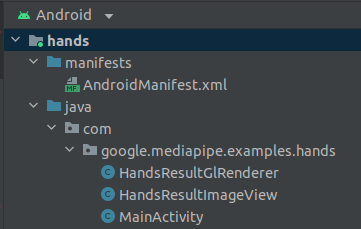
\includegraphics[width=0.5\textwidth]{images/struct_demo.png}
\end{figure}
\noindent Ovviamente, \texttt{MainActivity} corrisponde all'entry point dell'applicazione ed eredita infatti da \texttt{AppCompatActivity}.\\
\\
\noindent Nonostante noi ci siamo concentrati solo sull'input da streaming video, l'applicazione mette a disposizione 3 diverse modalità di acquisizione dell'input, rappresentate dall'enumerativo \texttt{InputSource} all'interno del quale troviamo \texttt{CAMERA}, \texttt{VIDEO} e \texttt{IMAGE}.\\


\section{Struttura del progetto}
\begin{figure}[H]
    \centering
    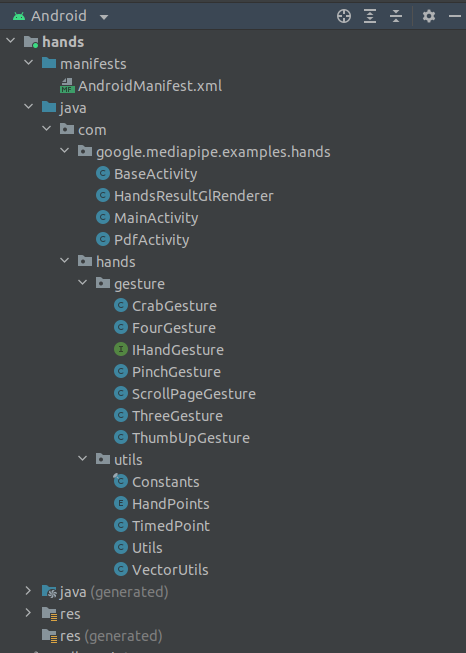
\includegraphics[width=0.8\textwidth]{images/struct_progetto.png}
\end{figure}
All'interno del package \texttt{hands/java/com/google/mediapipe/examples/hands} abbiamo potuto eliminare la classe \texttt{HandsResultImageView}, utile solo con acquisizione dell'input tramite immagine statica; mentre la classe \texttt{HandsResultGlRenderer}, per il rendering su schermo, è stata lasciata sostanzialmente inalterata.\\
Sono state invece applicate delle modifiche consistenti alla classe \texttt{MainActivity} (aggiungendo anche altre due classi \textit{Activity}) per implementare la logica applicativa.\\


\subsection{BaseActivity, MainActivity e PdfActivity}
Mentre prima era \texttt{MainActivity} ad ereditare da \texttt{AppCompatActivity}, ora questo avviene per \texttt{BaseActivity}, da cui erediteranno poi la classe \texttt{PdfActivity} e la nuova \texttt{MainActivity}.\\
Abbiamo scelto di adottare questa strategia implementativa per suddividere in modo chiaro e pulito le funzionalità esposte dalle due classi:
\begin{itemize}
    \item \texttt{MainActivity}: si occupa di definire il layout dell'applicazione nel caso in cui si voglia visualizzare su tutto lo schermo la propria mano, con alcune \texttt{TextView} per mostrare il riconoscimento di determinate \textbf{gesture}.
    \item \texttt{PdfActivity}: corrisponde al cuore dell'applicazione, definendo un layout nel quale è presente un file \texttt{pdf} da leggere ed una piccola vista della fotocamera interna dello smartphone. Quest'ultima ha lo scopo di mostrare all'utente il movimento della propria mano, tramite la quale avrà la possibilità di interagire con il file.
\end{itemize}
\noindent Entrambe le \textit{activities} hanno quindi lo scopo di mostrare la mano ed il riconoscimento di gesture, la prima \textit{"loggando"} l'eventuale riconoscimento, la seconda interagendo con il pdf.\\
Per fare questo, all'interno di ognuna, viene definito un \textbf{listener} che controlla continuamente l'eventuale associazione di un movimento della mano ad una gesture. Sono state infatti create 6 classi, una per gesture, che si occupano di effettuare il controllo sulla base dei \textbf{landmarks} passati in input dalle \textit{activities}.\\
\\
Prima di concentrarci su questE classi, di seguito vengono esposte caratteristiche più dettagliate di ognuna delle \textit{activitites} presentate sopra.

\subsubsection{BaseActivity}
Questa classe funge da contenitore per tutte quelle variabili e funzioni comuni sia a \texttt{MainActivity} sia a \texttt{PdfActivity} (perciò dichiarate con la clausola \texttt{protected}). Questa permette di evitare la ridondanza di codice.\\

\paragraph{Variabili} Alcune delle variabili comuni definite sono:
\begin{itemize}
    \item \texttt{Hands}, tramite la quale viene recuperato il \textbf{listener} nominato sopra, da cui poi otteniamo i risultati del mapping effettuato dalla pipeline di riconoscimento di MediaPipe.
    \item \texttt{InputSource}, che rappresenta la modalità di acquisizione dell'immagine (da noi sarà sempre \texttt{CAMERA}).
    \item \texttt{CameraInput}, che rappresenta la ricezione dell'input dalla fotocamera.
\end{itemize}
\noindent Abbiamo poi \texttt{SolutionGlSurfaceView$<$HandsResult$>$} e \texttt{HandsResultGlRenderer} per la definizione del layout e per il rendering.\\ 
Infine, sono presenti le istanze di tutte quelle classi che effettuano il rilevamento delle gesture, che, come detto in precedenza, sono necessarie ad entrambe le \texttt{activities}, anche se con scopi diversi.

\paragraph{Metodi} Essendo che questa classe eredita da \texttt{AppCompatActivity}, è necessario effettuare l'\texttt{override} dei seguenti metodi:
\begin{itemize}
    \item \texttt{onCreate}, accetta un \texttt{Bundle} in input, utilizzato per chiamare la \texttt{onCreate} della classe estesa. In Android Studio i \textit{Bundle} si utilizzano solitamente per il passaggio di dati da un attività all'altra: in questo caso abbiamo un istanza di uno stato salvato precedentemente (e.g. l'applicazione era stata messa in background). All'interno di questa funzione è solito definire il layout della pagina, ma abbiamo scelto di farlo solo nelle \textit{activities specializzate} che erediteranno da \texttt{BaseActivity}.
    \item \texttt{onPause}, nella quale viene chiamata la \texttt{onPause} della classe estesa per poi nascondere la visibilità del layout (\texttt{glSurfaceView}) e fermare infine il flusso video in input dalla fotocamera.
    \item \texttt{onResume}, dove dopo essere stata chiamata la \texttt{onResume} della classe estesa, si istanzia un nuovo \texttt{CameraInput} (passandogli l'\textit{activity} corrente) per poi settare un nuovo \textit{FrameListener}. Successivamente viene utilizzata l'istanza di \texttt{SolutionGlSurfaceView<HandsResult>} per chiamare il metodo interno \texttt{post}, passandogli la funzione interna \texttt{startCamera()} (il cui scopo è quello di inizializzare lo streaming video). In questo modo, tramite la \texttt{post} ereditata dalla classe \texttt{View}, viene eseguita la funzione passata ed esposto l'output nell'interfaccia utente.
\end{itemize}
\noindent Sono presenti poi ulteriori funzioni che vengono utilizzate da \texttt{MainActivity} e \texttt{PdfActivity} per inizializzare la pipeline di acquisizione dell'input e per terminarla. Verranno analizzate in seguito.



\subsubsection{MainActivity}
Abbiamo detto che lo scopo di questa \textit{activity} è quello di mostrare su schermo l'eventuale riconoscimento di determinate gesture. Perciò, oltre alle variabili definite nella classe estesa, le uniche variabili globali presenti sono una serie \texttt{TextView}, una per ogni gesture.\\
Viene effettuato l'\texttt{override} delle funzioni ereditate da \texttt{AppCompatActivity} e, mentre \texttt{onPause} e \texttt{onResume} chiamano solamente le relative funzioni della classe \texttt{BaseActivity}, la \texttt{onCreate} si occupa inoltre di \underline{inizializzare lo streaming video} e di definire il layout della pagina, istanziando anche un nuovo bottone per accedere alla funzionalità di interazione coi file \texttt{pdf}.\\
\\
Per quanto riguarda l'inizializzazione dello streaming video, vengono utilizzate due funzioni:
\begin{itemize}
    \item \texttt{setupLiveDemoUiComponents}, all'interno della quale viene definito un bottone per attivare lo streaming che, una volta cliccato, causerà la chiamata alla stessa funzione della classe estesa (il cui scopo è quello di fermare la pipeline di acquisizione attuale (nel caso in cui la modalità di acquisizione sia diversa da \texttt{CAMERA})). Successivamente, viene chiamata la funzione che implementa effettivamente la pipeline, mostrata qui sotto.
    \item \texttt{setupStreamingModePipeline}, questa funzione è divisa sostanzialmente in 3 parti, oltre ad una preliminare nella quale vengono inizializzate le \texttt{TextView}. \begin{enumerate}
        \item chiamata alla funzione \texttt{firstSetupStreamingModePipeline} di \texttt{BaseActivity} che crea delle nuove istanze di \texttt{HandsResultGlRenderer}, \texttt{Hands} e \texttt{glSurfaceView}. Tramite essa inizia lo streaming dalla fotocamera e, concorrentemente, la pipeline per il mapping dei \textbf{landamrks} della mano.
        \item settato il \textbf{listener} per il riconoscimento delle gesture, all'interno del quale vengono effettuate delle chiamate alle classi per il controllo e mostrato l'eventuale riconoscimento colorando le \texttt{Textview} definite prima.
        \item chiamata alla funzione \texttt{lastSetupStreamingModePipeline} di \texttt{BaseActivity} che chiama il metodo \texttt{post} di \texttt{glSurfaceView} visto in precedenza e definisce il nuovo \texttt{FrameLayout} con i dati trovati nella fase precedente.
    \end{enumerate}
\end{itemize}


\subsubsection{PdfActivity}
Il funzionamento di questa classe è analogo a quella mostrata in precedenza. Viene ovviamente differenziato il layout della pagina e, all'interno del \textit{listener} della funzione \texttt{setupStreamingModePipeline}, vengono associate le varie gesture riconosciute ad azioni che permettono di interagire con il file \texttt{pdf} che si sta visualizzando.
\chapter{Riconoscimento gesture}

\section{Introduzione alle tecniche utilizzate}

Ci siamo occupati di riconoscere due tipologie di gesture: statiche e dinamiche.\\
Gli strumenti utilizzati sono stati quelli appena spiegati nel \hyperref[chap:metodi]{\underline{capitolo precedente}}, come i vettori, 
la velocità e le distanze dei vari punti rispetto al centro del polso, che identifica la nostra origine.\\
La scelta di adottare le distanze dal polso rimane valida perché le dita si possono muovere solo di 180°, gli unici punti su cui porre attenzione sono quelli del pollice che spesso assumono la stessa distanza dal polso con gesture diverse:

\vspace{+ 15 px}
\begin{multicols}{2}
    \begin{multicolfigure}
        \centering
        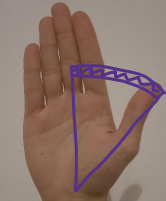
\includegraphics[width=0.956\textwidth]{images/pollici_1.png}
    \end{multicolfigure}
    \columnbreak
    \begin{multicolfigure}
        \centering
        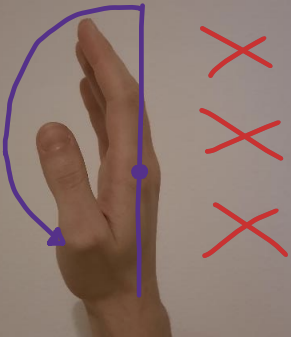
\includegraphics[width=\textwidth]{images/pollici_2.png}
    \end{multicolfigure} 
\end{multicols}
\vspace{+ 15 px}
  
\noindent Quindi la distanza punto-centro polso può essere utilizzata come discriminante, questione diversa sarebbe stata se le dita fossero state in grado di muoversi liberamente a 360°. Infine, ritornando alla problematica del pollice, in alcuni casi è stato necessario verificare se un dito preso in analisi fosse dritto o piegato.\\

\newpage
\section{Algoritmi per il riconoscimento}
Nella sezione che segue verrà mostrata la logica applicativa dietro il riconoscimento di ogni gesture.

\subsection{Gesture statiche}
Per tutte le gesture appartenenti a questa categoria è stata utilizzata la metodologia \textbf{a livelli}.
\subsubsection{Thumb up}
Per riconoscere il "\textit{pollice in su}" abbiamo scelto di prendere in analisi le punte di ogni dito della mano. Sono stati quindi misurati e testati empiricamente dei livelli che rappresentassero il movimento che volevamo. 
In particolare, abbiamo constatato che questi valori fossero i seguenti:
\begin{multicols}{2}
    \begin{multicolfigure}
        \centering
        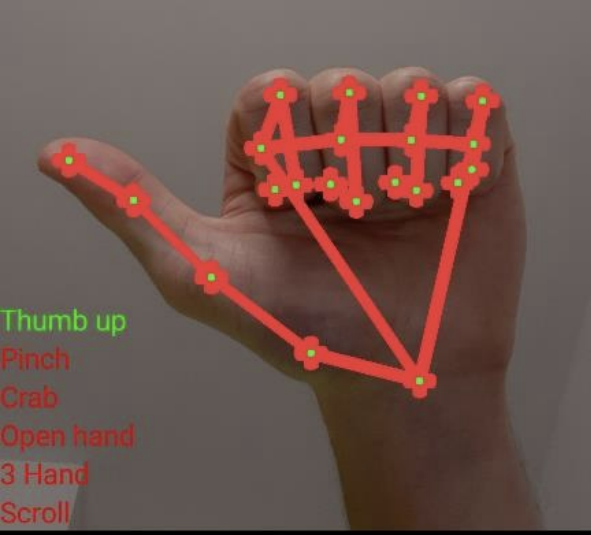
\includegraphics[width=\textwidth]{images/thumb_up.png}
    \end{multicolfigure}
    \columnbreak
    \begin{itemize}
        \item \texttt{HandPoints.THUMB\_TIP}: 52
        \item \texttt{HandPoints.INDEX\_TIP}: 35
        \item \texttt{HandPoints.MIDDLE\_TIP}: 29
        \item \texttt{HandPoints.RING\_TIP}: 27
        \item \texttt{HandPoints.PINKY\_TIP}: 29
    \end{itemize} 
\end{multicols}

\noindent Abbiamo poi introdotto un errore di 8 livelli per avere un buon trade-off tra precisione della posizione e flessibilità del riconoscimento.\\
\\
\noindent Infine, è stato inserito un ulteriore controllo per verificare che il pollice sia in posizione diritta (esteso). Questo è necessario per il motivo detto prima, secondo il quale i \textit{landmarks} del pollice spesso assumono la stessa distanza dal polso pur essendo in posizioni diverse.

\newpage
\subsubsection{Three Hand}
Per il simbolo "\textit{tre}", la tecnica è stata analoga al caso precedente.\\
I valori rilevati come punto di riferimento sono stati i seguenti:
\begin{multicols}{2}
    \begin{multicolfigure}
        \centering
        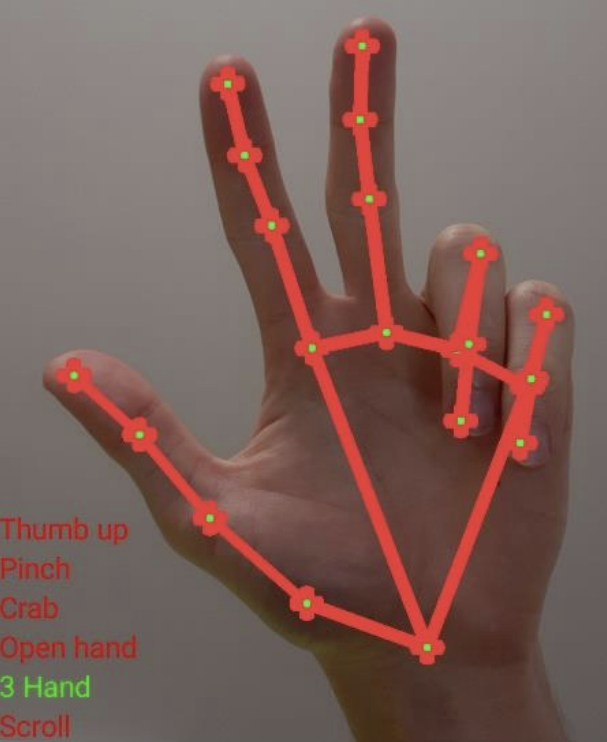
\includegraphics[width=\textwidth]{images/three_hand.png}
    \end{multicolfigure}
    \columnbreak
    \begin{itemize}
        \item \texttt{HandPoints.THUMB\_TIP}: 48
        \item \texttt{HandPoints.INDEX\_TIP}: 65
        \item \texttt{HandPoints.MIDDLE\_TIP}: 67
        \item \texttt{HandPoints.RING\_TIP}: 39
        \item \texttt{HandPoints.PINKY\_TIP}: 32
    \end{itemize} 
\end{multicols}
\noindent Anche qui, viene effettuato il controllo sul fatto che il pollice sia esteso.


\subsubsection{Four Hand}
Anche per il simbolo "\textit{quattro}", la tecnica è stata la stessa.\\
I valori rilevati come punto di riferimento sono stati i seguenti:
\begin{multicols}{2}
    \begin{multicolfigure}
        \centering
        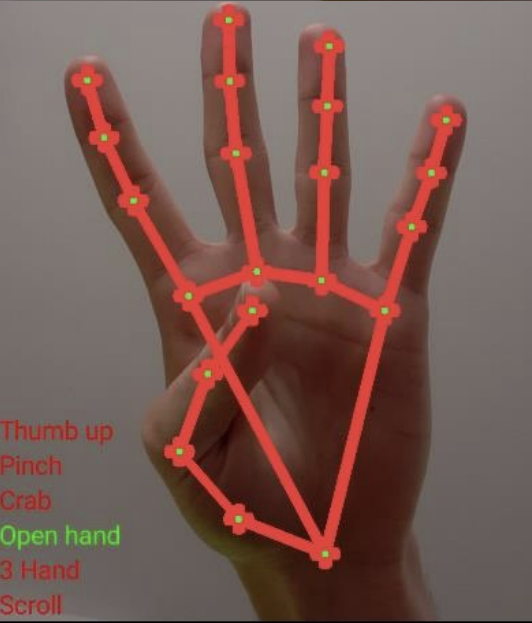
\includegraphics[width=\textwidth]{images/four_hand.png}
    \end{multicolfigure}
    \columnbreak
    \begin{itemize}
        \item \texttt{HandPoints.THUMB\_TIP}: 42
        \item \texttt{HandPoints.INDEX\_TIP}: 63
        \item \texttt{HandPoints.MIDDLE\_TIP}: 67
        \item \texttt{HandPoints.RING\_TIP}: 62
        \item \texttt{HandPoints.PINKY\_TIP}: 54
    \end{itemize} 
\end{multicols}


\subsection{Gesture dinamiche}

\subsubsection{Crab}
A differenza dei casi appena visti, qui ci si occupa di verificare che le punte del pollice e dell'indice si tocchino e che il pollice sia piegato.\\
Oltre a rilevare la gesture era necessario sapere di quanto si spostava la punta del pollice mentre il riconoscimento del gesto era valido. 
Essendo che Mediapipe offre anche dei valori già in forma di coordinate normalizzate rispetto allo schermo (\texttt{multiHandLandmarks}), è stato sufficiente andarsi a costruire un vettore con partenza il primo punto rilevato appena la gesture viene riconosciuta e come destinazione l'ultimo punto rilevato.\\
In questo modo abbiamo tracciato un vettore direzionato a rappresentare il nostro movimento.
\begin{figure}[H]
    \centering
    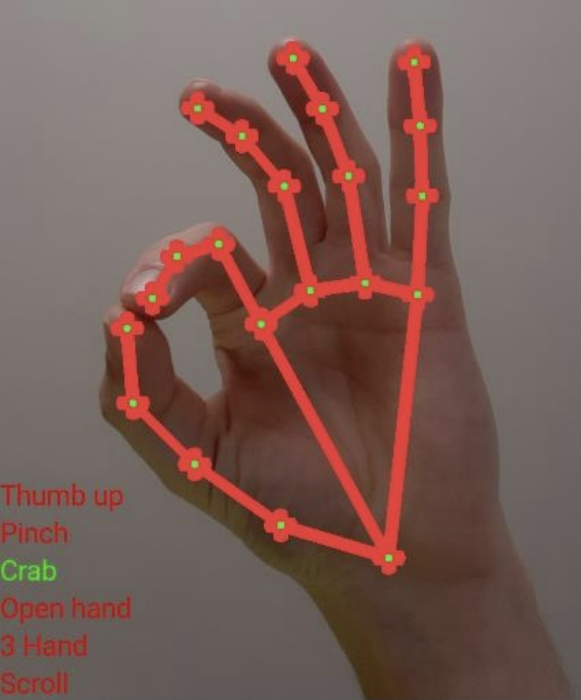
\includegraphics[width=0.6\textwidth]{images/crab.png}
\end{figure}
\noindent Il protocollo di riconoscimento impone che si inizi con la mano aperta, si chiudano pollice ed indice e li si muovano poi per definire il vettore di spostamento.

\newpage
\subsubsection{Pinch}
Per questa gesture viene utilizzata una metodologia ibrida.\\
Si verifica che la posizione delle punte delle dita medio, anulare e mignolo siano coerenti (a fronte di un margine di errore) coi seguenti livelli:
\begin{itemize}
    \item \texttt{HandPoints.MIDDLE\_TIP}: 29
    \item \texttt{HandPoints.RING\_TIP}: 27
    \item \texttt{HandPoints.PINKY\_TIP}: 29
\end{itemize} 
\noindent Succesivamente, si rileva la distanza tra la punta dell'indice e del pollice.
\begin{multicols}{2}
    \begin{multicolfigure}
        \centering
        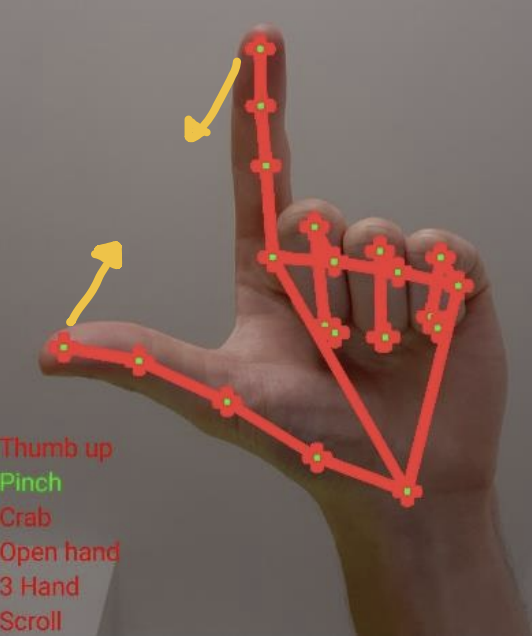
\includegraphics[width=0.9\textwidth]{images/pinch_1.png}
    \end{multicolfigure}
    \columnbreak
    \begin{multicolfigure}
        \centering
        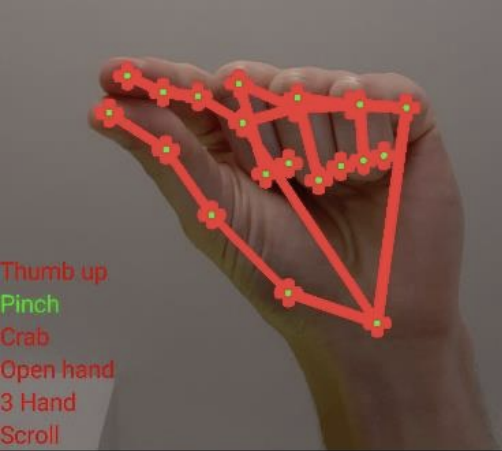
\includegraphics[width=1.1\textwidth]{images/pinch_2.png}
    \end{multicolfigure} 
\end{multicols}
\noindent Il protocollo di riconoscimento impone che si inizi con la mano a forma di \texttt{L} (come nell'immagine a sinistra).

\newpage
\subsubsection{Scroll}
Viene utilizzato il concetto di velocità.\\
Come verifica preliminare, si controlla che indice e medio siano le uniche due dita alzate (ovvero che i loro \textit{landmarks} siano quelli con una coordinata \texttt{y} minore). Inoltre, si verifica che il pollice sia piegato per non entrare in conflitto con la gesture \texttt{pinch}.\\
\\
\noindent Al primo riconoscimento, passati i controlli precedenti, si verifica che la posizione della punta del dito indice si trovi su un lato dello schermo e, in caso affermativo, si memorizza il valore della \texttt{x} della punta dell'indice per poi poterlo confrontare in un secondo rilevamento.\\
Infatti, se la punta dell'indice risulta essersi mossa nel lato opposto dello schermo con una velocità superiore ad una certa soglia, la gesture è riconosciuta.
\begin{multicols}{2}
    \begin{multicolfigure}
        \centering
        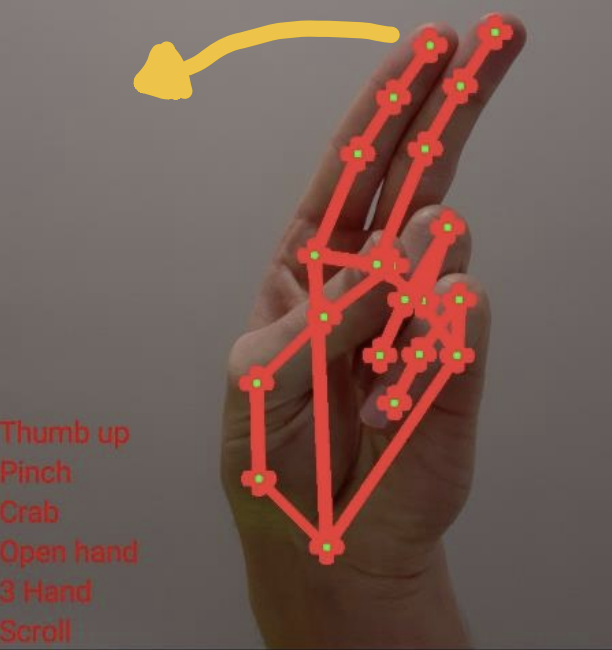
\includegraphics[width=\textwidth]{images/scroll_1.png}
    \end{multicolfigure}
    \columnbreak
    \begin{multicolfigure}
        \centering
        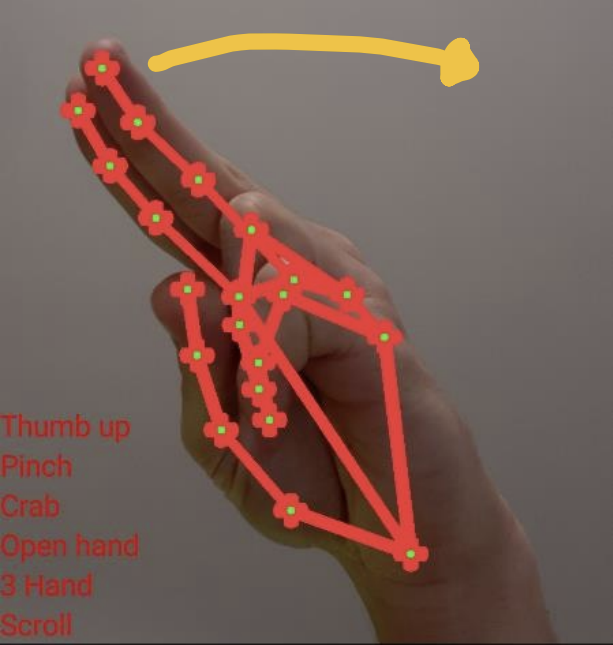
\includegraphics[width=\textwidth]{images/scroll_2.png}
    \end{multicolfigure} 
\end{multicols}
\chapter{Metodologie di riconoscimento delle gesture}
\label{chap:metodi}

Come già specificato in \hyperref[chap:landmarks]{\underline{MediaPipe Hands}}, il framework mette a disposizione due collezioni distinte di punti tridimensionali: 
\begin{itemize}
    \item la lista dei landmark a coordinate globali con origine nel centro geometrico approssimato della mano
    \item la lista dei landmark con coordinate X e Y normalizzate all'intervallo [0.0 - 1.0] per le dimensioni dell'immagine in input, la coordinata Z trova il suo centro nella posizione del landmark del polso
\end{itemize}

\noindent Abbiamo utilizzato entrambe le strutture per la rilevazione delle gesture, insieme a una combinazione delle le tecniche descritte di seguito, impiegando l'una o l'altra a seconda del tipo di azione alla quale la particolare gesture è collegata (vedi \ref{gesture}).

\section{Distanze tra landmark}

Il primo metodo che abbiamo implementato per discriminare una gesture dall'altra consiste semplicemente nel considerare la distanza tra landmark impiegando un sottoinsieme di punti rilevanti per la particolare gesture.

Abbiamo rilevato le distanze tra landmark caratterizzanti una particolare posizione delle dita che forma la gesture voluta in modo empirico, sfruttando opportune stringhe di log per visualizzare in tempo reale le distanze dei punti, per poi compilare una struttura dati usata come riferimento per identificare la gesture.

In seguito a queste analisi abbiamo notato, come ipotizzato in precedenza, le piccole ma non trascurabili fluttuazioni dei valori ottenuti dal framework, che impedivano un accurato riconoscimento della gesture; questo ha portato a considerare una soglia di errore sulle distanze rilevate, effettivamente individuando dei range di posizionamento delle dita che costituivano le gesture.

Aggiungendo nuove gesture alla nostra applicazione, abbiamo riscontrato un livello di inaccuratezza sempre più alto, manifestato nella forma di gesture rilevate contemporaneamente ad altre o, in certi casi, non rilevate affatto.

\section{Normalizzazione a livelli}

Dati i risultati della prima fase di test, abbiamo realizzato che molti fallimenti nella rilevazione di una gesture erano dovuti alla naturale differenza di dimensione tra le nostre mani.

Il passo successivo è stato quindi quello di trovare un modo per tentare di normalizzare le misure effettuate, questo ci ha portato a identificare, dopo una serie di prove, una distanza caratteristica da utilizzare come misura per uniformare le altre. Accordando sulla misura della distanza dalla punta del dito medio al landmark del polso, siamo riusciti a migliorare nettamente il riconoscimento di una determinata gesture effettuate da mani differenti.

Questa distanza è calcolata sommando le distanze tra i quattro landmark del dito medio (le tre falangi e la base) e la distanza tra la base e il landmark polso.

Abbiamo poi accoppiato questa tecnica con la mappatura delle misure a un range di livelli discreto, in modo da ridurre l'impatto dell'instabilità dei valori forniti dal framework, a scapito di un minimo livello di accuratezza, dopo diversi tentativi, abbiamo deciso di suddivedere la distanza scelta in 70 livelli, valore che ritiene una precisione sufficiente delle misure e mitiga gli effetti delle fluttuazioni.

\section{Lo spazio tridimensionale}

Le tecniche implementato fino ad ora non tengono veramente conto del fatto che le gesture hanno una forte caratteristica tridimensionale, in quanto riducono lo stato della mano a un insieme di parametri monodimensionali, abbiamo infatti notato che molte posizioni che vogliamo identificare presentano notevoli similitudini nello spazio delle distanze tra landmark.

Un parametro che abbiamo scelto di adottare nel sistema di riconoscimento è quello dell'allineamento nello spazio tridimensionale di un certo dito, o più in generale di un insieme di landmark.

Per ottenere questa informazione, abbiamo implementato una serie di funzioni di utilità che permettono di identificare il discostamento che una serie di punti ha dalla retta 3D formata da altri due punti dati; il calcolo di questa misura, unito a una lista di valori di errore ottenuti in modo sperimentale, permette di quantificare il livello di ripiegamento di un certo dito.

\begin{figure}[H]
    \centering
    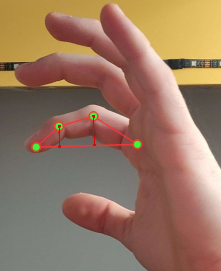
\includegraphics[width=0.3\textwidth]{images/mano_vettore.png}
\end{figure}

Grazie a questa tecnica, unita alle metodologie sopra descritte, siamo riusciti a ottenere una identificazione molto più accurata della posizione delle dita di una mano e a ridurre significativamente il grado di sovrapposizione tra gesture.

Anche in questo caso abbiamo implementato la normalizzazione a livelli delle misure effettuate, prendendo però in considerazione una distanza di riferimento variabile, ovvero la lunghezza di ogni falange del dito considerato.

\section{Rilevamento velocità e direzione}

L'utilità di un sistema di riconoscimento di gesture non si ferma soltanto alla rilevazione di posizioni statiche, è infatti desiderabile poter ottenere anche informazioni relative alla velocità e direzione di certi landmark significativi, utilizzando poi questi dati per abilitare l'utente a una gamma più vasta di interazioni.

Per una delle gesture implementate, si è reso necessario creare una apposita classe \texttt{TimedPoint}, che mette a disposizione funzionalità di calcolo della velocità media e della direzione tra due \texttt{TimedPoint}, questi dati vengono poi utilizzati per abilitare l'identificazione di gesture in seguito a un movimento definito a una certa velocità media.

Questi calcoli ci hanno permesso di definire gesture \textbf{dinamiche}, che devono essere rilevate \textbf{in seguito a un movimento} effettuato a una certa velocità e in una certa direzione, e non in seguito all'avverarsi di una posizione statica.

E' importante specificare che anche le gesture cosiddette \textit{statiche}, in certi casi vengono utilizzate per ottenere parametri che vengono poi applicati in particolari modi all'applicazione, il fatto che questi parametri sono dinamici non le categorizza come gesture dinamiche. 



\chapter{Funzionalità dell'applicazione}

Come detto durante l'analisi della struttura del progetto, la nostra applicazione è strutturata con due classi principali: \texttt{MainActivity} e \texttt{PdfActivity}. Questo ci permette di distinguere e separare le due funzionalità principali della nostra applicazione.

\begin{figure}[H]
    \centering
    %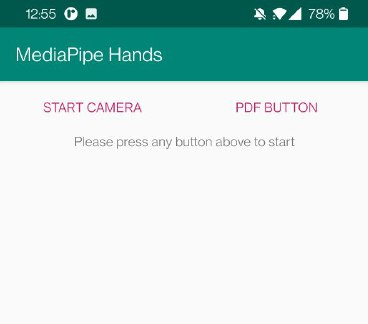
\includegraphics[width=0.7\textwidth]{images/homepage.png}
\end{figure}


\section{MainActivity}
Questa classe corrisponde all'entry point della nostra applicazione. All'interno di essa sono stati definiti due pulsanti: \texttt{StartCamera} e \texttt{PdfButton}.\\
Il primo permette di attivare la telecamera frontale 
del nostro dispositivo Android, previa autorizzazione dell'utente. In questo caso viene mostrato lo 
stream della videocamera in tempo reale, elaborato quasi istantaneamente dalle nostre 
implementazioni, in modo da ridurre il ritardo che ne potrebbe scaturire e dunque uno sfasamento 
temporale che porterebbe al lag della nostra applicazione.
\begin{figure}[H]
    \centering
    %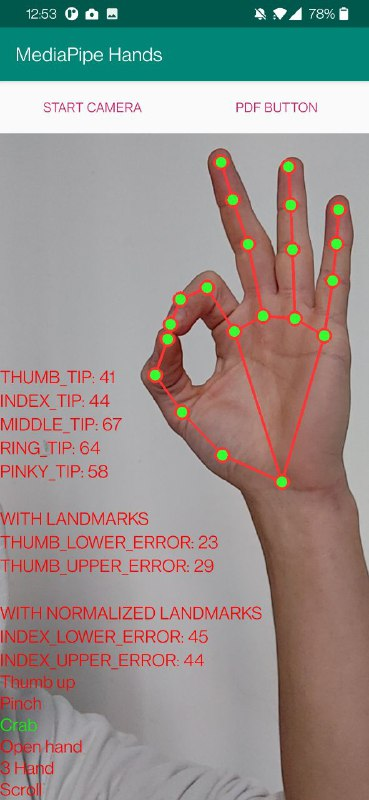
\includegraphics[width=0.7\textwidth]{images/startcamera.png}
\end{figure}

\noindent In questo scenario, attivando la videocamera, verrà presentato all'utente l'immagine della fotocamera interna con la sua mano mappata da 21 punti 
differenti (\textit{landmarks}), ovvero 4 punti per dito, che ci permettono di differenziare le varie falangi, e un punto per 
il polso che ci permette di riconoscere l'orientamento della mano e la profonfità relativa.\\
\\
\noindent Abbiamo utilizzato questa funzionalità per sperimentare le varie gesture da noi implementate, osservando nelle \texttt{TextView} da noi create
l'effettivo cambiamento delle coordinate dei punti che identificano le nostre dita, nonché il 
riconoscimento della gesture eseguita, la cui scritta verrà colorata di verde (rossa in origine).


\section{PdfActivity}
Dopo aver testato e dimostrato il corretto funzionamento del nostro applicativo, abbiamo deciso di applicare 
quanto appena appreso a contesti quotidiani in modo da renderlo utile e funzionale per eventuali 
utilizzatori. Abbiamo dunque applicato le nostre gesture alla lettura e all'interazione con un file pdf.\\
\\
\noindent Cliccando infatti sul quarto ed ultimo bottone della \texttt{MainActivity}, ovvero \textit{"Pdf Button"}, andiamo 
tramite un \texttt{Intent} a creare una nuova schermata, chiamata \texttt{PdfActivity}, che svolge le funzionalità 
appena espresse.\\
In questa schermata abbiamo creato 2 View separate: una, la principale, per 
mostrare il pdf (effettuato utilizzando un \texttt{PdfViewer} ottenuto grazie alla libreria esterna 
\texttt{com.github.mhiew}), l'altra, di dimensioni ridotte e posta sopraelevata in basso a destra, per 
gestire la videocamera frontale e per consentire, dunque, all'utente, di vedere le gesture 
effettuate.
\begin{figure}[H]
    \centering
    %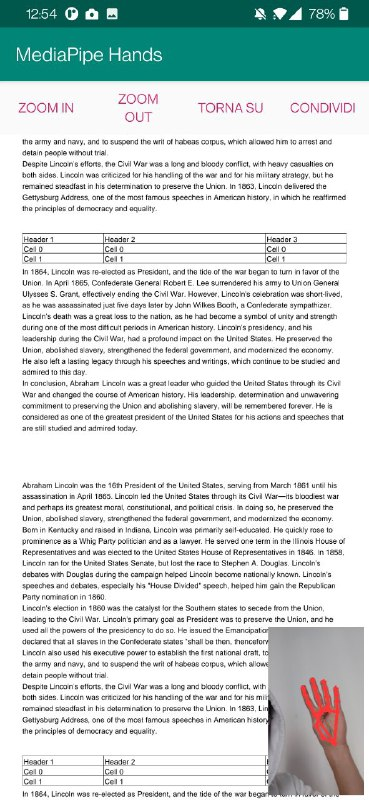
\includegraphics[width=0.7\textwidth]{images/pdfactivity.png}
\end{figure}

\subsection{Mapping delle gesture con azioni del pdf}
Abbiamo così applicato il lavoro effettuato nel nostro MainActivty al pdf, mappando le gesture definite in precedenza a determinati azioni sul file pdf.

\begin{itemize}
    \item Gesture statiche \begin{itemize}
        \item \textbf{Thumb up}: apertura del prompt di condivisone del pdf mostrato.
        \item \textbf{Three hand}: comparsa di un \texttt{AlertDialog} per la scelta del pdf da visualizzare (creati una sola volta al primo avvio tramite la libreria \texttt{iTextPdf} e poi mantenuti in memoria).
        \item \textbf{Four hand}: scroll continuo verticale del pdf, che scende di 40 pixel al secondo, in modo da emulare la lettura del file stesso.
    \end{itemize}
    \item Gesture dinamiche \begin{itemize}
        \item \textbf{Crab}: rende possibile muoversi all'interno del pdf (scroll) in qualsiasi direzione.
        \item \textbf{Pinch}: si incrementa o diminuisce il valore dello zoom sul pdf aumentando o riducendo la distanza tra indice e pollice.
        \item \textbf{Scroll}: permette di cambiare pagina verso sinistra o verso destra, in base alla direzione del movimento.
    \end{itemize}
    
\end{itemize}


\chapter{Conclusione}

\section{Analisi delle performance}

\subsection{Limiti dell'applicazione}

\subsubsection{Limiti imposti da MediaPipe}
\begin{enumerate}
    \item \textbf{Framerate limitato}: comprensibile contando che siamo su dispositivi mobile, meno elaborazioni facciamo meno batteria viene consumata.
    \item \textbf{Dati imprecisi quando non tutte le dita vengono mostrate}: se si mostra una gesture che non espone tutte le dita bene in vista (pollice in su) e si muove la mano cambiando punto di vista, le coordinate rilevate dalla libreria non rimangono coerenti.
    \item \textbf{Applicazione basata su immagini ben illuminate}: se nello stream video manca di luminosità l'accuratezza del rilevamento cala drasticamente (problema noto nel mondo di computer vision)
\end{enumerate}

\subsubsection{Limiti della nostra soluzione}
\begin{enumerate}
    \item \textbf{Consumo batteria relativamente elevato}: per una app mobile porre attenzione ai consumi è fondamentale, la nostra applicazione consuma un 2\% ogni 4 minuti circa su una batteria 4000mAh. Questo consumo è comprensibile considerando il lavoro che svolge; un fattore critico è rappresentato dall'impossibilità di avere momenti di stand-by in quanto il tracking delle mani lavora anche quando non vi sono mani da riconoscere, portando i momenti morti (dove non accade nulla ma l'applicazione è attiva) ad una fonte di spreco risorse.
    \item \textbf{Lentezza di gesture}: essendo il framerate limitato bisogna effettuare le gesture con calma per stare dietro alle elaborazioni.
    \item \textbf{Gesture non eccessivamente elastiche}: l'applicazione utilizza le proporzioni usando come riferimento la lunghezza fisica del dito medio fino ad arrivare al centro del polso; tutte le altre misure rilevate sono comparate con quella. Dal punto di vista teorico dovrebbe funzionare su tutte le mani, ma, dovendo discriminare le gesture in modo abbastanza rigido per evitare che gesture differenti si confondano tra di loro, per effettuare correttamente i segni in alcuni casi le dita vanno orientate in un modo specifico (\texttt{crab} gesture $=$ il pollice deve essere particolarmente inclinato (vincolo posto per non confondere tale gesture con il \texttt{pinch})).
\end{enumerate}

\subsection{Profiling con Android Studio}
I dati presentati in seguito sono stati raccolti dal profiler di Android Studio su un dispositivo con le seguenti specifiche:
\begin{itemize}
    \item \textbf{GPU}: ARM MALI-G72 MP3 (850MHz)
    \item \textbf{CPU}: Octa-core, 2 processori: 4x 2.3GHz ARM Cortex-A73 (Quad-core), 4x 1.7GHz ARM Cortex-A53 (Quad-core)
    \item \textbf{RAM}: 6GB
\end{itemize}

L’ambiente di sviluppo Android Studio offre un comodissimo pannello per verificare il consumo relativo delle risorse utilizzate dalla propria applicazione. La seguente immagina riassume i nostri valori rilevati:

%% inserimento immagini profiling con commenti e analisi %%
\begin{figure}
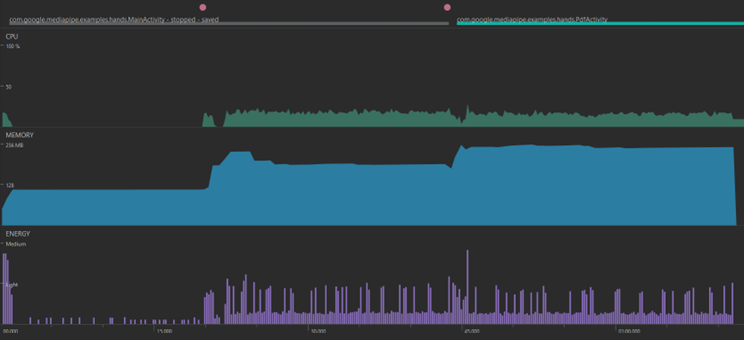
\includegraphics[width=\textwidth]{images/profiling_app.png}
\end{figure}

Il profiling è suddiviso in tre sezioni che corrispondono alle tre pagine visualizzabili, in ordine: pagina home, pagina start camera e pagina PdfReader. Nel complesso non abbiamo misurazioni stravolgenti, la CPU viene utilizzata mediamente il 17\% del suo potenziale quando il tracking delle mani è attivato (start camera e PdfReader), mentre alla home page dove non succede nulla giustamente il consumo è nullo tranne che al suo primo caricamento. La memoria viene utilizzata principalmente nella gestione dei Pdf con picchi massimi di 256MB. Mentre sotto il punto di vista dei consumi Android Studio pone nell’asse delle ordinate tre livelli: Light, Medium e High; al di là dei cambi di pagina che vengono etichettati come Medium, il consumo generale viene considerato Light. Siccome questo dato non ci ha orientato più di tanto per capire se tale consumo possa essere considerato tollerabile, come accennato nel paragrafo precedente, abbiamo provato molto empiricamente a verificare di quanto scendeva il livello di batteria durante l’utilizzo dell’app realizzando un calo di un 2\% ogni 4 minuti con una batteria 4000mAh. Facendo lo stesso con la nota app Instagram il consumo è risultato differente, con un uso di un 2\% ogni 7 minuti, quindi messa a confronto la nostra applicazione consuma il doppio. Ipotizzando uno scenario realistico dove consideriamo il 100\% di batteria di un utente intenzionato a studiare con la nostra applicazione(con le specifiche di dispositivo citate prima)  e dedicando un 80\% alla nostra applicazione si ottiene una durata massima di 2 ore e mezza. Esito non malvagio ma pensare che dopo 2 ore e mezza di lettura il dispositivo diviene inutilizzabile non è molto invitante, i ruoli però si potrebbero invertire se cambia il contesto dove si utilizza il riconoscimento gesture.



\section{Opinioni e sviluppi futuri}
La possibilità di poter interagire con un dispositivo tramite una videocamera introduce un metodo alternativo di 
interfacciamento con la macchina. Nel corso degli anni i computer si sono evoluti sempre di più mentre il 
metodo per interagire con essi è rimasto sempre lo stesso: la tastiera.\\
Solo nell'ultimo decennio, grazie ad una 
sufficiente maturazione della tecnologia, si è cominciato concretamente a pensare a mezzi differenti per comunicare 
con i dispositivi. D'altronde siamo di fronte ad una situazione dove due macchine computazionali potenti (cervello e 
computer) nella loro collaborazione sono ostacolate dall'interfacciamento Input/Output che gli si pone in mezzo ed è
per questo che soluzioni che rendono più immediato e naturale il trasferimento dei dati saranno probabilmente l'argomento 
di discussione principale degli anni a seguire.\\
\\
\noindent Il nostro team si è occupato di analizzare un “proof-of-concept” di una 
applicazione PdfReader gestita non dall'interfacciamento proposto dello schermo touch ma dalla videocamera 
frontale che rileva specifiche gesture. Svolgendo i test finali siamo rimasti soddisfatti del risultato; l'unico tallone 
d'Achille è il fatto di avere un riconoscimento gesti in alcuni casi abbastanza rigido, dovuto proprio ai dati non molto 
precisi che Mediapipe pone quando non tutte le dita vengono mostrate.\\
Un'idea di risoluzione sarebbe porre due videocamere che riprendono due angolazioni diverse e poi 
elaborate insieme per ricostruire la posizione delle dita. Questa proposta però non avrebbe molti punti a favore 
considerando che nei dispositivi già sul mercato non sarebbe compatibile oltre al fatto di svolgere il doppio delle 
elaborazioni, ma per prodotti non mobile ancora da inserire sul mercato come una lavagna LIM che adotta questa 
tecnica non sarebbe una idea da scartare a priori.\\
\\
\noindent In questo progetto ci si è limitati a gestire un pdf, ma una volta che la logica di gesture detection è stata messa a punto 
e anche il consumo migliorato ecco che cambiare scenario diviene immediato: è sufficiente collegare le gesture a determinate 
azioni. Un esempio potrebbe essere la simulazione del cursore tramite gesture, permettendo quindi di navigare nell'interfaccia proposta 
dallo schermo. Combinando poi il riconoscimento delle mani con altri tipi di riconoscimenti (face, body, ...) potrebbe 
nascere qualcosa di interessante. Rimanendo però nel mondo mobile, potendo consumare poca batteria e di 
conseguenza non avendo una grande potenza computazionale a disposizione, il framerate limitato non permette di riconoscere accuratamente gesture dinamiche 
veloci, ciò nonostante si riescono a realizzare applicazioni con interazioni più naturali rispetto ai classici pulsanti. Sarebbe valido proporre una soluzione 
dove l'applicazione non elabora direttamente i dati, ma delega un server remoto con una potenza di calcolo molto maggiore.
\end{document}
